\chapter{\label{chap:spelunkbots}SpelunkBots}

\begin{mdframed}[backgroundcolor=green!20]
Reestruturar este capítulo (pegar informações do tutorial e da API):
\begin{itemize}
    \item
		Breve descrição
    \item
        Como funciona: código-fonte do Spelunky, modos de programar os bots (C++
		e GML), processo de compilação, modos de execução (Marathon e
		TestLevel)
	\item
		Detalhar envio de comandos para o bot
    \item
		Detalhar informações disponibilizadas (três categorias: Node Data, Enemy
		Data e Object Data) e sistema de fog of war
	\item
		Exemplo de esqueleto de um bot (funções que precisam ser implementadas:
		Initialise e Update)
\end{itemize}
\end{mdframed}

Utilizando o código-fonte de Spelunky, Daniel Scales e Thomas Thompson, da
Universidade de Derby no Reino Unido, criaram o
\textit{SpelunkBots}\cite{SPELUNKBOTSPAPER}, um
\textit{framework} que permite a programação de \textit{bots} para o jogo
Spelunky. Um dos objetivos dos criadores é utilizar a aplicação para criar uma
competição de inteligência artificial para o jogo.

A \textit{API} possibilita que o desenvolvedor resgate informações de objetos
estáticos e dinâmicos contidos no ambiente do jogo, como o terreno, a
posição de tesouros, armadilhas e inimigos. Contudo, o objetivo da \textit{API}
disponibilizada por SpelunkBots é fazer com que a informação recebida pelo
\textit{bot} se assemelhe ao máximo com a percepção de um jogador humano.  Para
tal, o \textit{framework} implementa um sistema de \textit{fog of war},
limitando o conhecimento do ambiente que pode ser obtido pela inteligência
artificial. Para objetos estáticos, uma vez que o jogador visualizou o objeto,
ele poderá receber informações sobre ele permanentemente. Para objetos
dinâmicos, o \textit{bot} só poderá receber informações sobre eles se os mesmos
estiverem sendo visualizados por ele. A figura \ref{fig:spelunkbots-fow} ilustra
um exemplo de funcionamento do sistema, onde as áreas marcadas com o valor ``0''
representam um terreno transponível, enquanto as áreas com o valor ``1''
representam terreno intransponível. As áreas intransponíveis com o fundo
acinzentado correspondem ao sistema de \textit{fog of war}, cujas informações
não estão disponíveis pois tal área ainda não foi explorada pelo \textit{bot}.

\begin{figure}[htb!]
\centering
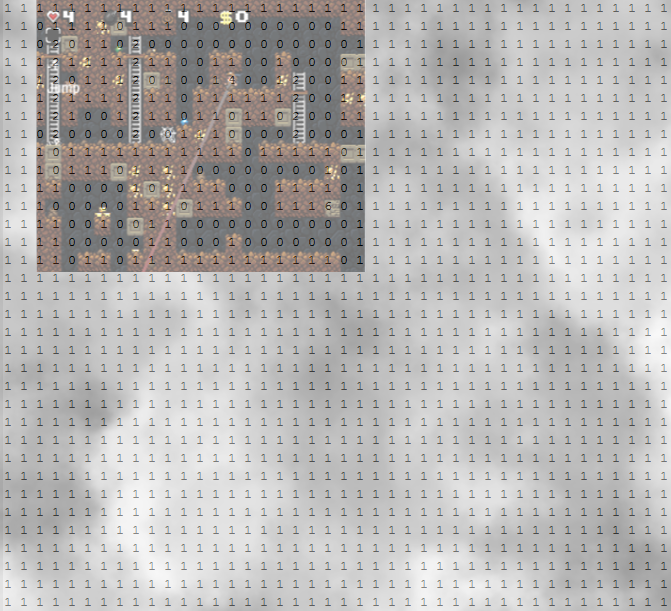
\includegraphics[width=.65\textwidth]{fig/spelunkbots-fow.png}
\caption {\label{fig:spelunkbots-fow}Visualização do sistema de \textit{fog of
war} demonstrando a diferença de informação recebida de elementos dentro e fora
do campo de visão do jogador.}
\end{figure}

\section{Utilização da \textit{API}}

É possível desenvolver \textit{bots} que fazem uso da \textit{API}
utilizando a linguagem GML (sigla para \textit{Game Maker Language}) ou
através da linguagem C++, ficando a critério do desenvolvedor a escolha da
linguagem. A única restrição que existe quanto ao uso de C++ dá-se no fato
de que a linguagem necessita de um processo de compilação através de uma
ferramenta externa, não sendo gerenciada diretamente pelo \textit{Game
Maker}. A figura \ref{fig:spelunkbots-usage-diagram} mostra a relação entre
o jogo, a \textit{API} e as possíveis linguagens de programação para se
utilizar. O código do Spelunky teve de ser modificado de forma a poder
interagir com o código do SpelunkyBots que, por sua vez, faz o uso de uma
solução de \textit{DLLs} escritas em C++ para fazer a interação com o jogo
através de código escrito em C++.

\begin{figure}[htb!]
\centering
\includegraphics[width=.65\textwidth]{fig/spelunkbots-usage-diagram.png}
\caption {\label{fig:spelunkbots-usage-diagram}Diagrama exibindo a relação
entre o jogo Spelunky, a API SpelunkyBots e as linguagens de programação que
podem ser usadas para a interação com o jogo.}
\end{figure}

A \textit{API} permite uma interação completa com o jogo através do uso
das variáveis expostas pelo
\textit{framework}\footnote{http://spelunkbots.com/wp-content/uploads/2015/02/SpelunkBots-API-A-Getting-Started-Tutorial.pdf}.
Com elas, é possível fazer o controle da movimentação do bot, bem
como identificar o tipo de terreno em que se está pisando e os inimigos que
aparecem em seu campo de visão. Além disso, também são disponibilizadas
informações sobre as armadilhas que podem atrapalhar o jogador. Por fim,
existem variáveis que permitem um melhor controle das informações relativas ao
\textit{bot}, como o posicionamento no eixo X e no eixo Y, se o \textit{bot}
encontra-se virado para a esquerda ou para a direita, entre outros. O uso dessas
variáveis torna possível a implementação de técnicas de inteligência artificial
no jogo Spelunky. O apêndice \ref{appendix:spelunkbots-variables} faz um
detalhamento maior de todas essas variáveis.
